\chapter{Sorption}\label{appSec:Sorption} 

\Cref{appfig:Kd_SAPV_C} shows the relationship between each of carbon content ($\log~C$), $\log~SA/PV$ and $\log~SA/PV/C$, now as a function of $\log~K_d$ (normalized to 1 $\mu g~L^{-1}$). This figure shows that a linear relationship exists between $\log~K_d$ and $\log~SA/PV/C$, and that no such relationship is present for carbon content and the SA/PV ratio individually. 

\begin{figure}[htb]
    \centering
    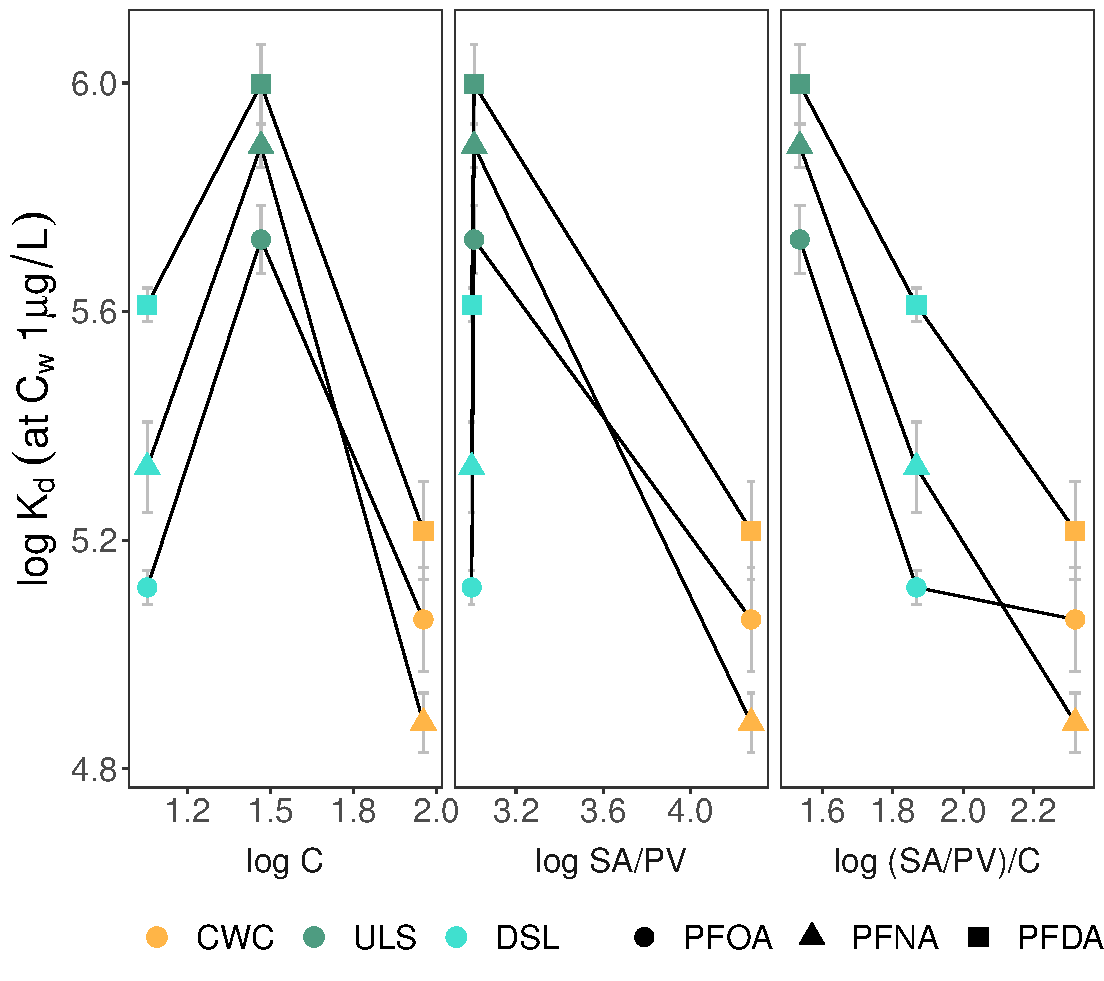
\includegraphics[width=0.8\textwidth]{R/figs/SAPV_C_Kd1ugL_plot.pdf}
    \caption{The correlation of $\log~K_d$ vs. (a) log C (b) log SA/PV (c) log (SA/PV)/C using BET for SA and BJH for PV by biomass feedstock. The points are discrete measurements, and the lines have been added to indicate trends. Error bars are the propagated standard error of $\log~K_F$ and $n$.}
    \label{appfig:Kd_SAPV_C}
\end{figure}

\begin{table}[ht]
\caption{$log~K_d$ for the soil (S) used in the batch shaking tests with a PFCA cocktail and single-spiked PFOA.}
\centering
\label{apptab:soil_Kd}
\begin{tabular}{llllr} \toprule
         & \multicolumn{4}{c}{blank}                                \\ \cline{2-5} 
Compound & type        & log Kd & log Kd se & \multicolumn{1}{l}{n} \\ \midrule
PFPeA    & S cocktail &        &           & 3                     \\
PFHxA    & S cocktail & 2.34   & 3.29      & 3                     \\
PFHpA    & S cocktail & 2.17   & 3.00      & 3                     \\
PFOA     & S cocktail & 2.72   & 4.35      & 3                     \\
PFNA     & S cocktail & 2.57   & 4.63      & 3                     \\
PFDA     & S cocktail & 2.55   & 5.19      & 3                     \\
PFOA     & S single    & 2.82   & 3.90      & \multicolumn{1}{l}{3} \\ \bottomrule
\end{tabular}
\end{table}


\begin{table}
\caption{Freundlich sorption coefficients and standard errors for isotherms. $log~K_F$ for the soil samples are the collective partition coefficients for soil and biochar because. All $K_F$ data are in units of $\mathrm{(\mu g/kg)/(\mu g/L)^{n_F}}$.}
\centering
\adjustbox{max width=\textwidth}{%
\begin{threeparttable}
\label{apptab:summary_stats_all}
\begin{tabular}{lllllllll} \toprule
\multicolumn{1}{c}{Compound} & \multicolumn{1}{c}{Biochar} & \multicolumn{1}{c}{type} & \multicolumn{1}{c}{$log~K_F$} & \multicolumn{1}{c}{se $log~K_F$} & \multicolumn{1}{c}{$n_F$} & \multicolumn{1}{c}{se $n_F$} & \multicolumn{1}{c}{$r^2$} & \multicolumn{1}{c}{$p$} \\ \midrule
PFPeA & CWC & BC\_S\_mix & \multicolumn{1}{c}{\textbf{}} & \multicolumn{1}{c}{\textbf{}} & \multicolumn{1}{c}{\textbf{}} & \multicolumn{1}{c}{\textbf{}} & \multicolumn{1}{c}{\textbf{}} & \multicolumn{1}{c}{\textbf{}} \\
PFHxA & CWC & BC\_S\_mix & 3.05 & 0.95 & 0.61 & 0.39 & 0.38 & \textgreater{}0.05 \\
PFHpA & CWC & BC\_S\_mix & 3.30 & 0.23 & 0.46 & 0.14 & 0.73 & * \\
PFOA & CWC & BC\_S\_mix & 3.25 & 0.48 & 0.77 & 0.18 & 0.82 & * \\
PFNA & CWC & BC\_S\_mix & 3.84 & 0.28 & 0.60 & 0.10 & 0.89 & * \\
PFDA & CWC & BC\_S\_mix & 4.31 & 0.18 & 0.57 & 0.06 & 0.95 & ** \\
PFOA & CWC & BC\_S\_sing & 3.45 & 0.21 & 0.88 & 0.09 & 0.96 & ** \\
PFPeA & CWC & BC\_sing & 3.98 & 0.36 & 0.56 & 0.33 & 0.30 & \textgreater{}0.05 \\
PFHxA & CWC & BC\_sing & 4.59 & 0.50 & -0.14 & 0.26 & 0.04 & \textgreater{}0.05 \\
PFHpA & CWC & BC\_sing & 4.44 & 0.05 & 0.59 & 0.11 & 0.80 & ** \\
PFOA & CWC & BC\_sing & 5.06 & 0.08 & 0.39 & 0.05 & 0.90 & *** \\
PFNA & CWC & BC\_sing & 4.88 & 0.04 & 0.65 & 0.04 & 0.98 & *** \\
PFDA & CWC & BC\_sing & 5.22 & 0.07 & 0.45 & 0.04 & 0.94 & *** \\
\addlinespace
PFPeA & DSL & BC\_S\_mix &  &  &  &  &  &  \\
PFHxA & DSL & BC\_S\_mix & 4.54 & 0.30 & 0.18 & 0.15 & 0.33 & \textgreater{}0.05 \\
PFHpA & DSL & BC\_S\_mix & 4.10 & 0.19 & 0.09 & 0.15 & 0.10 & \textgreater{}0.05 \\
PFOA & DSL & BC\_S\_mix & 4.91 & 0.06 & 0.39 & 0.03 & 0.97 & *** \\
PFNA & DSL & BC\_S\_mix & 5.10 & 0.06 & 0.35 & 0.03 & 0.97 & *** \\
PFDA & DSL & BC\_S\_mix & 5.48 & 0.04 & 0.35 & 0.03 & 0.98 & *** \\
PFOA & DSL & BC\_S\_sing & 5.08 & 0.10 & 0.46 & 0.08 & 0.90 & * \\
PFPeA & DSL & BC\_sing & 4.25 & 0.74 & 0.14 & 0.38 & 0.06 & \textgreater{}0.05 \\
PFHxA & DSL & BC\_sing & 3.30 & 0.15 & 1.12 & 0.11 & 0.93 & *** \\
PFHpA & DSL & BC\_sing & 4.67 & 0.06 & 0.57 & 0.09 & 0.86 & *** \\
PFOA & DSL & BC\_sing & 5.12 & 0.02 & 0.60 & 0.02 & 0.99 & *** \\
PFNA & DSL & BC\_sing & 5.33 & 0.03 & 0.80 & 0.07 & 0.94 & *** \\
PFDA & DSL & BC\_sing & 5.61 & 0.02 & 0.61 & 0.02 & 0.99 & *** \\
\addlinespace 
PFPeA & ULS & BC\_S\_mix &  &  &  &  &  &  \\
PFHxA & ULS & BC\_S\_mix & 4.39 & 0.13 & 0.32 & 0.06 & 0.86 & ** \\
PFHpA & ULS & BC\_S\_mix & 4.12 & 0.13 & 0.14 & 0.10 & 0.35 & \textgreater{}0.05 \\
PFOA & ULS & BC\_S\_mix & 5.00 & 0.05 & 0.39 & 0.03 & 0.98 & *** \\
PFNA & ULS & BC\_S\_mix & 5.22 & 0.04 & 0.37 & 0.03 & 0.97 & *** \\
PFDA & ULS & BC\_S\_mix & 5.62 & 0.04 & 0.37 & 0.03 & 0.97 & *** \\
PFOA & ULS & BC\_S\_sing & 5.16 & 0.03 & 0.62 & 0.03 & 0.99 & *** \\
PFPeA & ULS & BC\_sing & 4.10 & 0.13 & 0.67 & 0.16 & 0.74 & ** \\
PFHxA & ULS & BC\_sing & 4.80 & 0.06 & 0.34 & 0.09 & 0.72 & ** \\
PFHpA & ULS & BC\_sing & 5.98 & 0.17 & 1.08 & 0.11 & 0.93 & *** \\
PFOA & ULS & BC\_sing & 5.73 & 0.02 & 0.65 & 0.05 & 0.95 & *** \\
PFNA & ULS & BC\_sing & 5.89 & 0.02 & 0.71 & 0.03 & 0.99 & *** \\
PFDA & ULS & BC\_sing & 6.00 & 0.04 & 0.35 & 0.05 & 0.86 & *** \\ \bottomrule
\end{tabular}
\begin{tablenotes}
\item Significant codes: *** $\sim$ 0.001, ** $\sim$ 0.01, * $\sim$ 0.05
\end{tablenotes}
\end{threeparttable}}
\end{table}

